\documentclass[aspectratio=169]{beamer}
\usepackage{tikz}
\usepackage{graphicx}
\usepackage{listings}
\usepackage{xcolor}
\usepackage{hyperref}
\usepackage[spanish,es-noquoting]{babel}

\lstset{
  basicstyle=\ttfamily\small,
  keywordstyle=\color{blue},
  stringstyle=\color{red},
  commentstyle=\color{gray},
  showstringspaces=false
}
% Minimal look
\usetheme{Warsaw}
%\setbeamertemplate{headline}
\setbeamertemplate{footline}{
  \leavevmode%
  \hbox{%
    % Left: Section name
    \begin{beamercolorbox}[wd=.33\paperwidth,ht=2.25ex,dp=1ex,left]{author in head/foot}%
      \hspace*{2ex}\insertsection
    \end{beamercolorbox}%
    % Center: Presentation title
    \begin{beamercolorbox}[wd=.34\paperwidth,ht=2.25ex,dp=1ex,center]{title in head/foot}%
      \insertshorttitle
    \end{beamercolorbox}%
    % Right: Slide numbers
    \begin{beamercolorbox}[wd=.33\paperwidth,ht=2.25ex,dp=1ex,right]{date in head/foot}%
      \insertframenumber{} / \inserttotalframenumber\hspace*{2ex}
    \end{beamercolorbox}%
  }%
  \vskip0pt%
}

\usecolortheme{default}
\usefonttheme{serif}
\graphicspath{{../}{./}}
\setbeamertemplate{caption}[numbered]

% Title info
\title[ PromptLibrary Jurídica]{ PromptLibrary Jurídica}
\subtitle{ Construye el activo de IA más valioso de tu práctica (Módulo 3)}
\author{Ricardo Reyes-Jimenez}
\institute{Universidad de La Sabana}
\date{\today}

% Background image for title slide
\usebackgroundtemplate{
  \tikz\node[opacity=0.3]{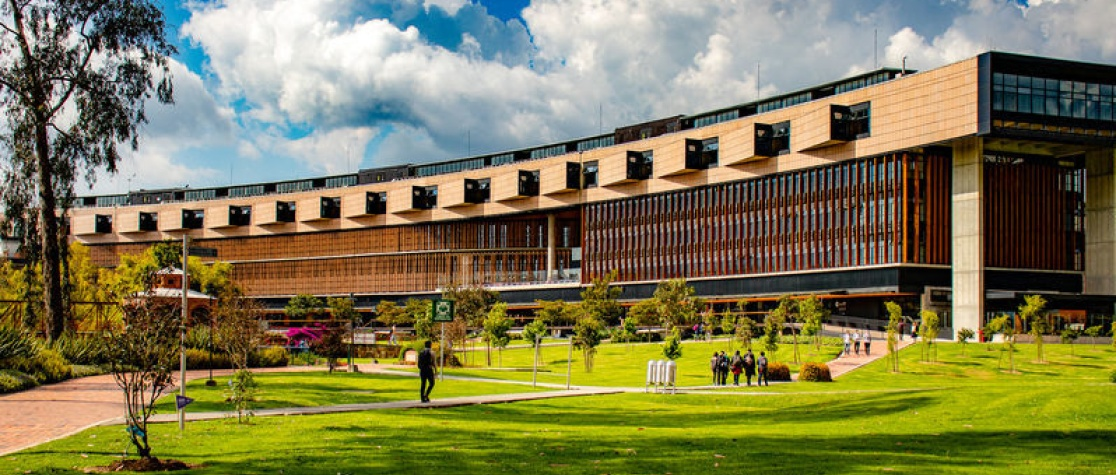
\includegraphics[width=\paperwidth,height=\paperheight]{Images/UniSabana.jpg}};
}

\begin{document}

% Title slide
\begin{frame}
  \titlepage
\end{frame}

% Reset background for normal slides
\usebackgroundtemplate{}


\begin{frame}{Objetivos de la Sesión (Día 1 \& 2)}
\begin{itemize}
  \item Entender el concepto y valor de una PromptLibrary corporativa.
  \item Diseñar iterativamente prompts fundacionales por rol (Litigio, Consultoría, etc.).
  \item Estrategia de crecimiento: De una herramienta agnóstica (ej. Word/Excel) a repositorios escalables (SharePoint).
  \item Mantenimiento y gobernanza del sistema en el tiempo.
  \item Taller Práctico: Creación colaborativa de la versión 1.0 de su biblioteca.
\end{itemize}
\end{frame}


\begin{frame}{¿Qué es una PromptLibrary y por qué importa?}
\begin{itemize}
  \item \textbf{Definición:} Un repositorio centralizado, probado y categorizado de instrucciones (prompts) listas para usar.
  \item \textbf{El Problema:} La ``Ceguera del Prompt''. Un asociado gasta 30 minutos logrando que la IA resuma bien un expediente, y ese conocimiento se pierde cuando cierra la pestaña.
  \item \textbf{La Solución:} Escalar el conocimiento. Si el asociado documenta ese prompt, los otros 50 abogados de la firma lo usarán mañana ahorrando 25 horas hombre \cite{murray2024}.
\end{itemize}
\end{frame}


\begin{frame}{Diseño Colaborativo: Empezando Simple (Día 1)}
\textbf{Framework Agnóstico (No necesitas software caro)}
\begin{itemize}
  \item \textbf{Fase 1 (Arranque):} Un simple documento de Word, Excel o Notion.
  \item \textbf{Estructura Básica por entrada:}
\end{itemize}
1. \textbf{Nombre del Prompt:} Ej. \textit{Resumen Ejecutivo de Sentencia (Laboral)}.
2. \textbf{Objetivo:} Para qué sirve y para qué NO sirve.
3. \textbf{El Prompt (Texto a copiar):} Con espacios en blanco tipo `[Insertar Texto Aquí]`.
4. \textbf{Versión y Autor:} Ej. \textit{v1.2 por Juan Pérez}.
\end{frame}


\begin{frame}{Evolución del Sistema: De lo Personal a SharePoint}
\textbf{Cómo Escalar (Fase 2 y 3)}
\begin{itemize}
  \item \textbf{Fase 1 (Personal):} Cada abogado tiene su propio ``Bloc de notas'' con sus trucos.
  \item \textbf{Fase 2 (Compartido - Agnóstico):} Un Excel en OneDrive / Google Sheets donde el equipo sube sus hallazgos.
  \item \textbf{Fase 3 (Institucional - SharePoint / Intranet):}
  \begin{itemize}
    \item Creación de un repositorio oficial en SharePoint con etiquetas (tags), buscador, e integración con Microsoft 365.
    \item Control de versiones y ``Prompts Aprobados'' por el Comité de Innovación.
  \end{itemize}
\end{itemize}
\end{frame}


\begin{frame}{Gobernanza y Sostenibilidad (Día 2)}
\textbf{¿Cómo evitar que la biblioteca muera en 3 meses?}
\begin{itemize}
  \item \textbf{El Comité de Revisión:} Asignar un ``Líder de IA'' por área de práctica \cite{sal2024}.
  \item \textbf{Actualización Constante:} Los modelos cambian (ChatGPT de hoy no responde igual que el de hace 6 meses). Los prompts deben auditarse cada trimestre.
  \item \textbf{Incentivos:} Premiar al abogado que más contribuya con prompts que ahorren tiempo (Gamificación).
\end{itemize}
\end{frame}


\begin{frame}{Taller Práctico: Construye tu V1.0}
\textbf{Dinámica en Grupos (Roles: Litigio, Asesoría, Sector Público):}
1. Identificar las 3 tareas más repetitivas de su área.
2. Diseñar en vivo un mega-prompt (usando los frameworks del Módulo 2) para cada tarea.
3. Documentarlos en una plantilla agnóstica (ej. tabla de Word).
4. Exposición: Un integrante simula la ``venta'' de este prompt al resto de la firma.
\end{frame}



\begin{frame}[allowframebreaks]{Referencias}
  \bibliographystyle{apalike}
  \bibliography{references}
\end{frame}

\end{document}